\section{Evaluation}

\subsection{Implementation of Transfer Learning}
In our first implementation, as shown in figure \ref {fig:xceptiona}, we feed an image to Xception model and took the average pooling of the last layer from Xception, and then we used a classification layer directly to classify the image. We used the cross-entropy loss for training. For this approach, we experimented by freezing the weights from Xception and by training it from scratch. 

\begin{figure}[h]
 \centering
  \begin{subfigure}[b]{\linewidth}
 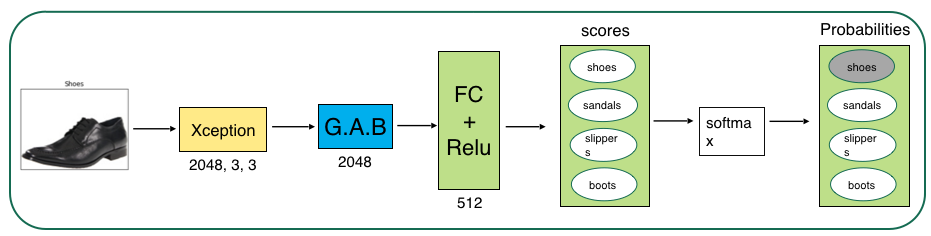
\includegraphics[width=\linewidth]{figs/xception_1.png}
  \caption{Version 1}
  \label{fig:xceptiona}
  \end{subfigure}
    \hfill
  \begin{subfigure}[b]{\linewidth}
 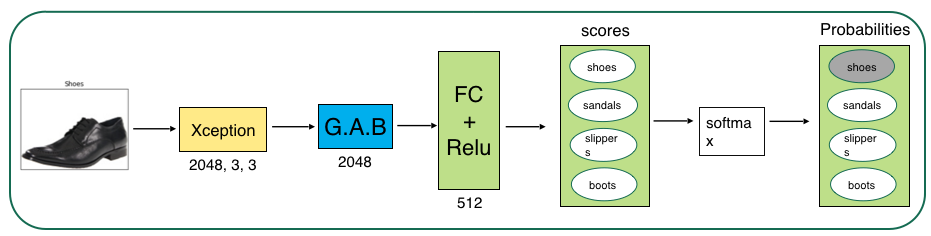
\includegraphics[width=\linewidth]{figs/xception_1.png}
 \caption{Version 2}
  \label{fig:xceptionb}
  \end{subfigure}
    \hfill    
 \caption{Implemented transfer learning architectures.}
 \label{fig:xception}
\end{figure}

On the second implementation, as shown in figure \ref{fig:xceptionb}, we froze learned weights from Xception but we added a fully connected layer before the prediction layer. For this fully connected, We used 512 Victor dimension because we wanted to match it with the best embedding size of our implementation for siamese network for the comparison. 

We used Adam optimizer with learning rate of 0.001 for all transfer learning approaches.

\subsection{Implementation of Siamese Network}

The architecture of our implementations of the siamese network is shown as in figure \ref{fig:model}. Our network consists of a batch input layer and a deep CNN followed by L2 normalization, which results in the image embedding. This is followed by a loss function during training. Note that the siamese network was designed originally for calculating the similarity between images, not the image classification. Normally, it would have a distance function to compute the similarity between the two embedding vectors as the final outputs. However, our project is for the image classification problem, so we add one more fully connected layer on top of that and trained it to predict the class of the embeddings (instead of the image). 

\begin{figure}[h]
  \centering
  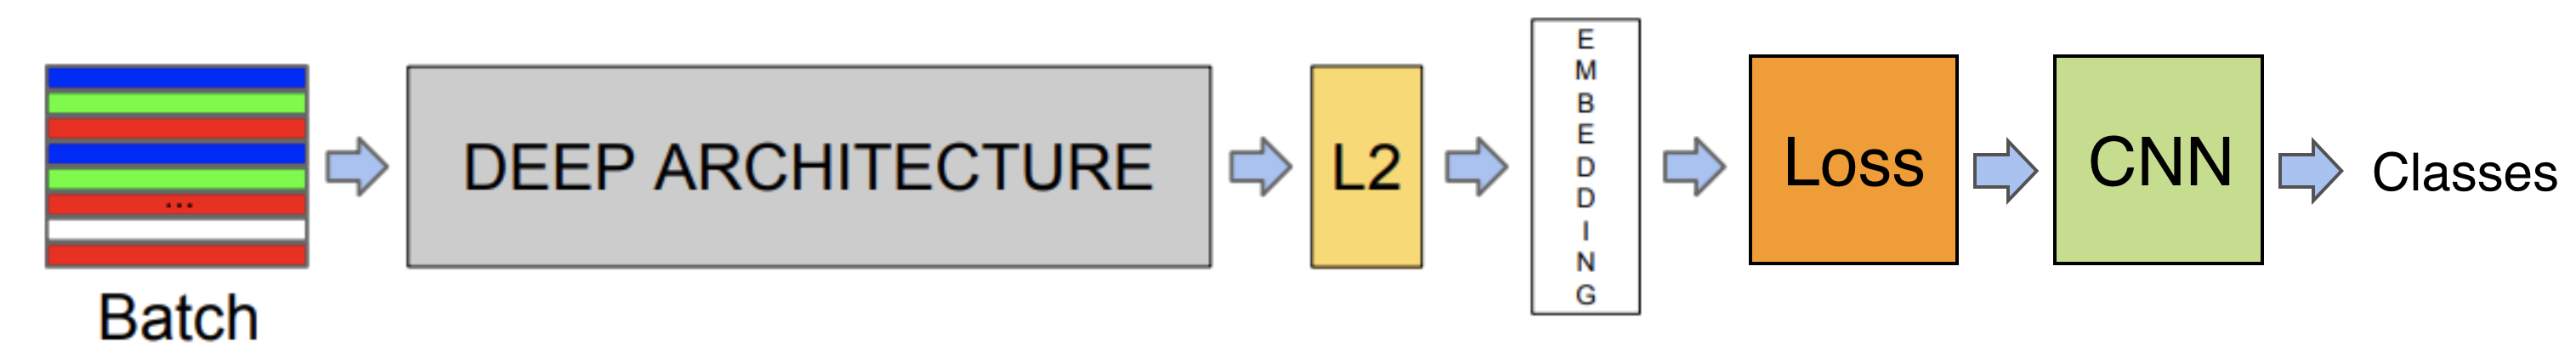
\includegraphics[width=\linewidth]{figs/model.png}
  \caption{The architecture of our model.}
  \label{fig:model}
\end{figure}

In this project, we implemented three variants of the siamese network. The first one is with contrastive loss, and the second one is with triplet loss. The third one is the combination of transfer learning and the one with triplet loss.

For the implementation of contrastive loss, we build the model and implement the loss function by ourselves using Keras and Tensorflow. The implementation can be partitioned into three steps: 1) generating image pairs, 2) construct the architecture of the siamese neural network, 3) using contrastive loss to train the model. We adopt a simple strategy to make the image pairs. The positive sample is picked randomly from the same category as the anchor, and label with 1. On the other hand, we grab the negative sample randomly from classes that are different from the anchor and label it with 0. Figure \ref{fig:pairs} shows the examples of the positive and negative pairs. 

\begin{figure}[h]
  \centering
  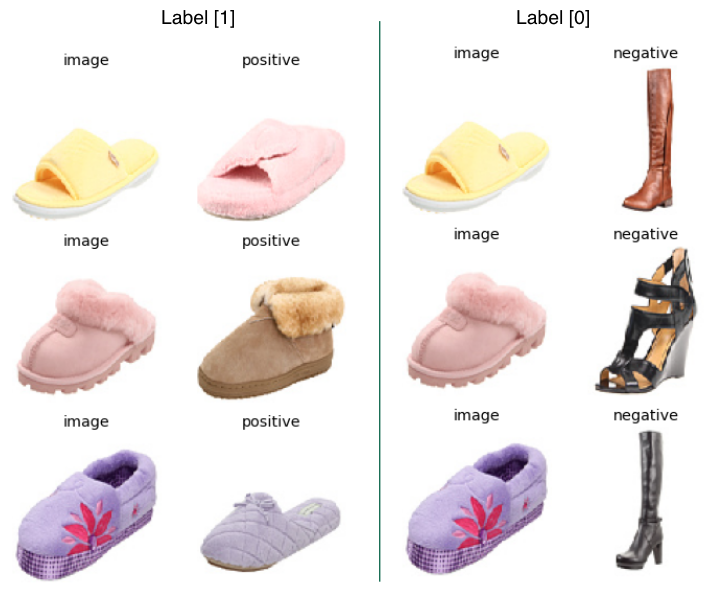
\includegraphics[width=0.9\linewidth]{figs/pairs.png}
  \caption{Examples of the positive and negative pairs.}
  \label{fig:pairs}
\end{figure}

For the implementation of triplet loss, we implement it by calling the TripletSemiHardLoss function in TensorFlow Addons. As shown in the paper \cite{schroff2015facenet}, the best results are from Semi-Hard triplets. This implementation contains three steps that are similar to the contrastive loss one. And we used the same strategy to make the triplets. The only difference is that we use the offline mining approach for the first implementation, while the online mining approach for the second one. Offline mining means that pairs are defined at the beginning of the training. Online mining means that triplets are defined for every batch during the training. And the latter one has been proved in better training efficiency and performance.

The CNN model in our implementations is represented in figure \ref{fig:cnn}. The hidden layers consist of convolutional layers, pooling layers, fully connected layers, and normalization layers (ReLU). All the parameters we used for training are as shown in the figure.  

\begin{figure}[h]
 \centering
 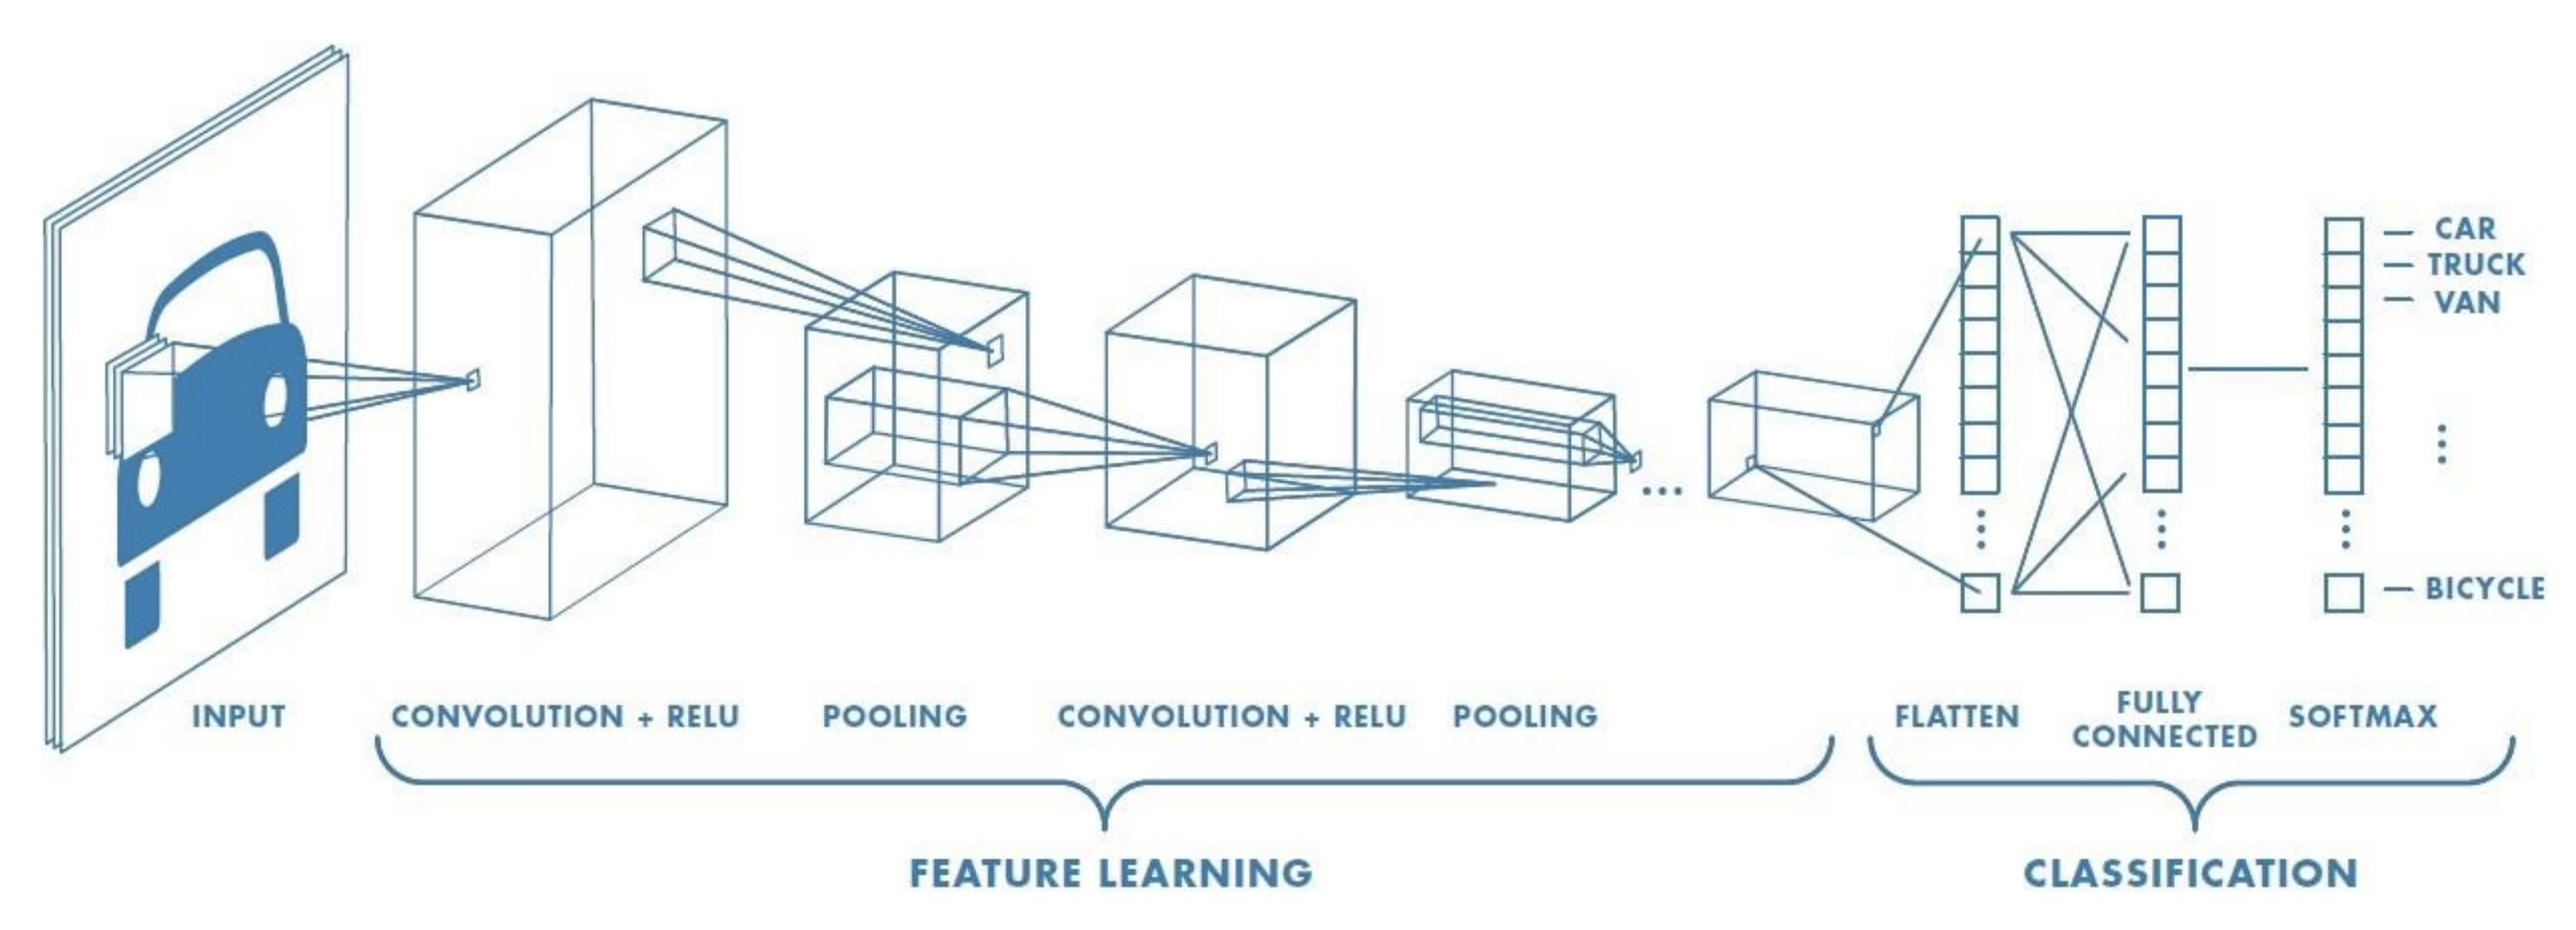
\includegraphics[width=\linewidth]{figs/cnn.png}
 \caption{The Convolutional Neural Network (CNN) in our implementations.}
 \label{fig:cnn}
\end{figure}

Furthermore, to improve the performance of the siamese network, we implemented another version with transfer learning. As shown in the figure, we used the Xception to extract the features firstly, followed by a global average pooling layer, and applied two dense layers on top of that. And this model is trained with the triplet loss. The implementation details are showed in figure \ref{fig:xception_cnn}. 

We used Adam optimizer with learning rate of 0.001 for all Siamese Network approaches. 

\begin{figure}[h]
  \centering
  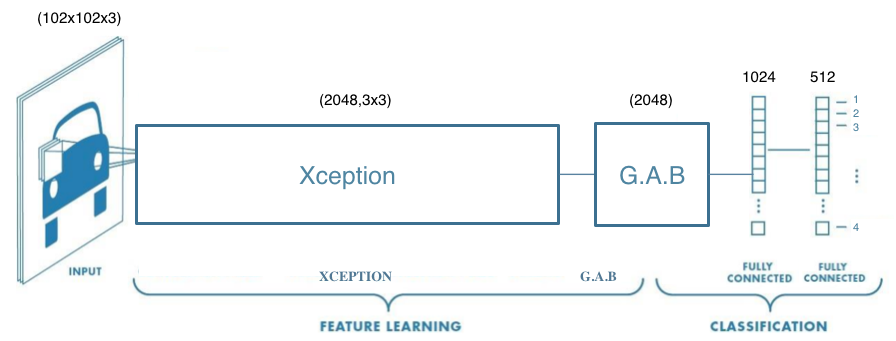
\includegraphics[width=\linewidth]{figs/xception_cnn.png}
  \caption{Applying  Xcepetion into our implementation.}
  \label{fig:xception_cnn}
\end{figure}

\subsection{Analysis and Results}
In this project, we have implemented three variants of transfer learning and three variants of the siamese network, as we mentioned in the last section. In this section, we compare the results of all the variants based on the classification accuracy and the time-consume. All our experiments are executed on the Cheaha supercomputer with a single GPU. 

The description and diagrams in 5.1 and 5.2 report our final model and hyperparameters. However, we have gone through a long process of model engineering and hyperparameter tuning to reach this final implementation. The following paragraphs describes this process step by step.
Step 1: building the simplest transfer learning model to identify our baseline. We turned several hyperparameters including optimizers (Adam and SGD with 0.9 momentum), learning rate (0.01, 0.001), and number of epochs (5, 10, 20, 30).
Step 2: building the CNN model to extract features for Siamese network. We used inputs size of 64x64, 102x102, and 102x136 (the original image size). The last two yields the same results in most experiments so we selected 102 X 102 as the input size for all experiments. Of course, with three channels since the images are of RGB color. Thin, we examine variance models.
- 2 layers of (conv, relu, maxpooling, dropout) with and without batch normalization and with different hyperparameters like number of filters, kennel size, polling size, and dropout rates. This is followed by a flatten layer and 1 or two dense layers. For the last dense (embedding) layer, we used 48, 64, and jumped to 512 where we get our best accuracy.
- 3 and 4 layers of (conv, relu, maxpooling, dropout) with increasing filters without padding. This is followed by a global average pooling instead of flatten layer and single dense layers. This approach led to overfitting no matter what hyperparameter tuning that we have tried.
Therefore, we went with the first approach with simple convolutions followed by flatten and 2 dense layers. We use the same CNN architecture to build the siamese network which we tested using contrastive and triplet loss.
Step 3: adding a single dense layer for Xception (transfer learning) and also training all layers in  Xception model.
Step 4: we combined transfer learning with siamese network by adding 1 and 2 dense layers on top of extracted features from exception and use the triplet loss to train our last model.

Table \ref{table:resultA}  summarizes the results of these six implementations trained on the dataset with 1500 images per category. T0 is the implementation that directly classifying the features extracted from Xception. T1 is the implementation that adds a single fully connected layer before the prediction. We observe that this leads to a 1\% decrease in performance. Most likely the large dense vector leads to over-fitting. We also trained Xception from scratch on this data set as shown in T2, and it improved the results by around 4\% when compared to T0. As shown in the figure \ref{fig:acc_ter}, it's clear that T2 is the best one among these three variants. Note that we've also made a comparison of the total time taken of the training, as depicted in the figure \ref{fig:time_ter}. The most interesting thing is that the time-consuming of each variant is roughly increasing linearly for these three variants. That means the time taken for each layer of the Xception is almost the same. 

\begin{table}[ht]
    \caption{Summary of the results on 1500 images per category} 
    \centering 
    \begin{tabular}{c c c c} 
    \hline\hline 
    
    model & Accuracy \% & Epochs & Time (mins)  \\% inserts table
    \hline % inserts single horizontal line
    Xception (T0) & 91.8 & 20 & 1.8 \\% inserting body of the table
    Xception+dense (T1) & 90.7 & 20 & 3.5 \\% inserting body of the table
    Xception All (T2) & 95.1 & 10 & 5.4 \\% inserting body of the table
    Our Siamese+Con. Loss (S0) & 92.57 & 32 & 6 \\% inserting body of the table
    Our Siamese+Triplet. Loss (S1) & 91.02  & 20& 2 \\% inserting body of the table
    Xception+Siamese (S2) & 95.85 & 10 & 2 \\% inserting body of the table
    \hline 
    \end{tabular}
\label{table:resultA} % is used to refer this table in the text
\end{table}

\begin{figure}[h]
  \centering
  \begin{subfigure}[b]{0.48\linewidth}
  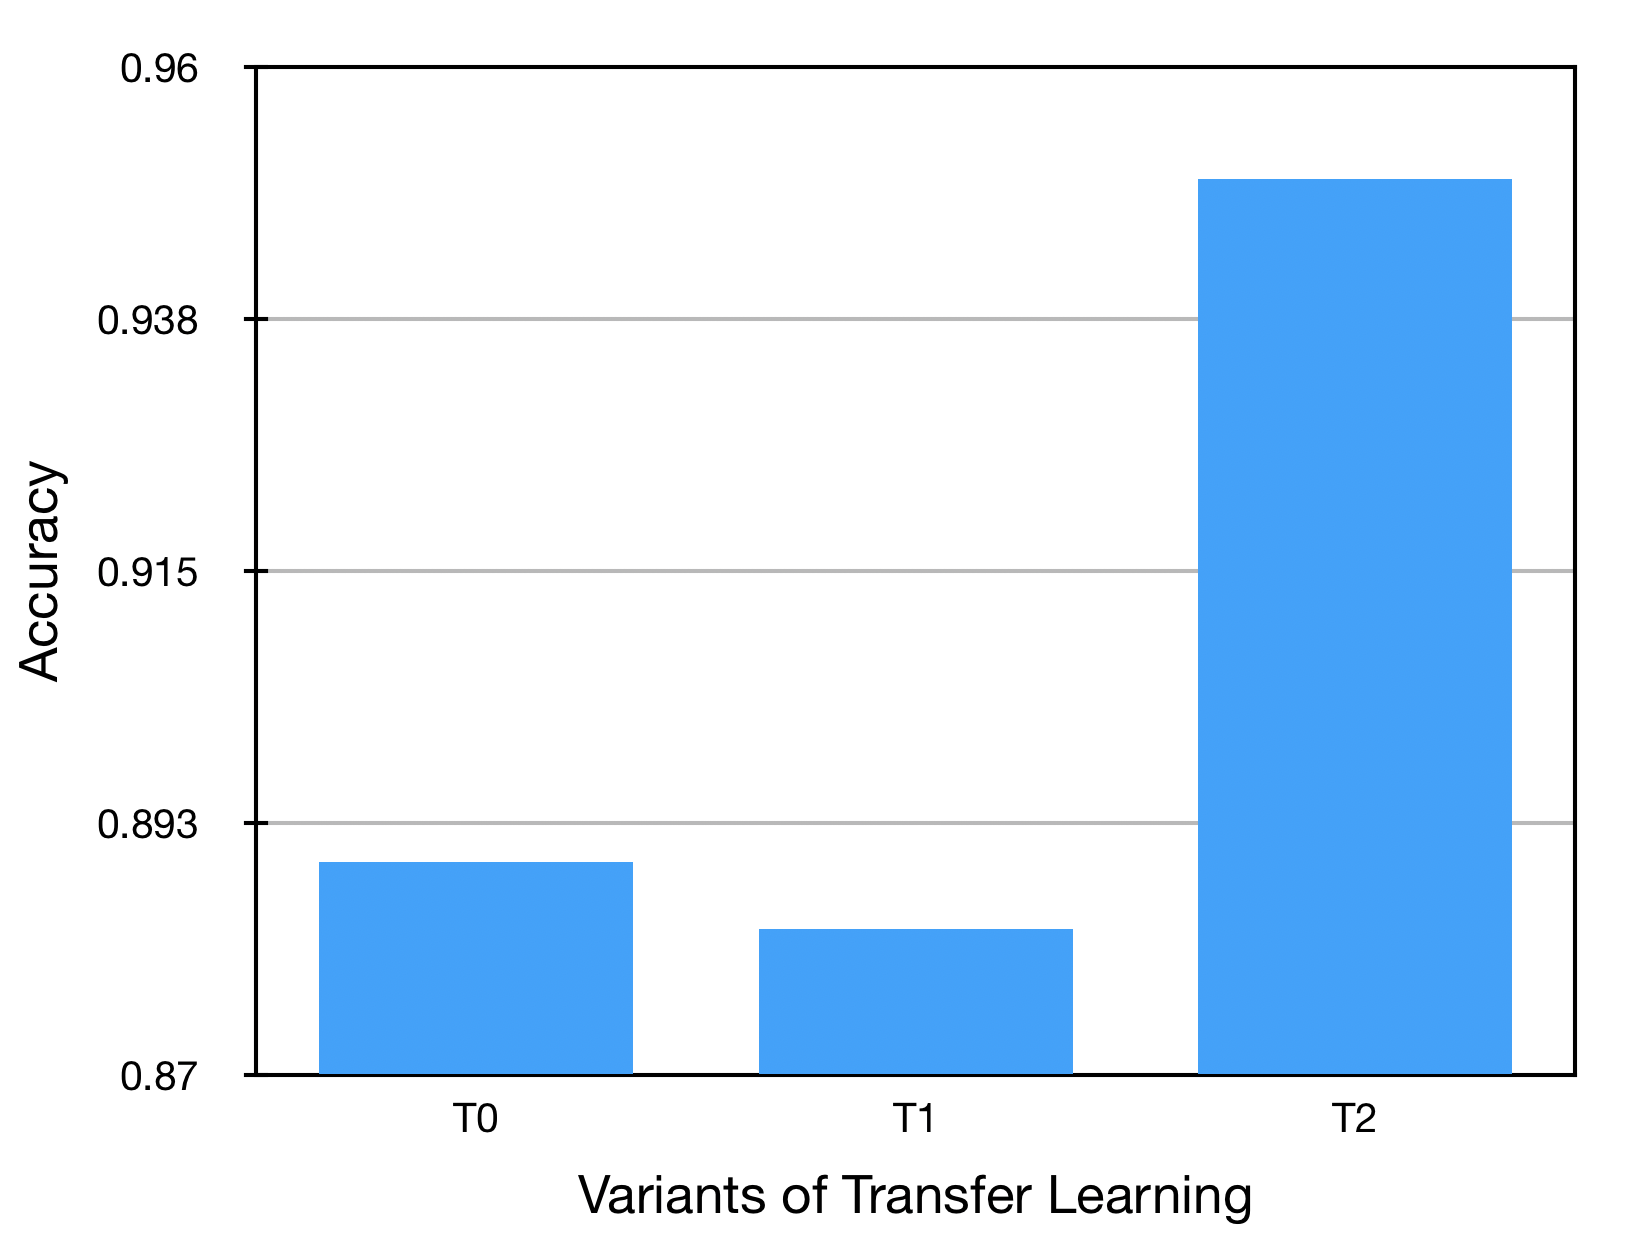
\includegraphics[width=\linewidth]{figs/acc_ter.png}
  \caption{Accuracy comparison}
  \label{fig:acc_ter}
  \end{subfigure}
  \hfill
   \begin{subfigure}[b]{0.48\linewidth}
   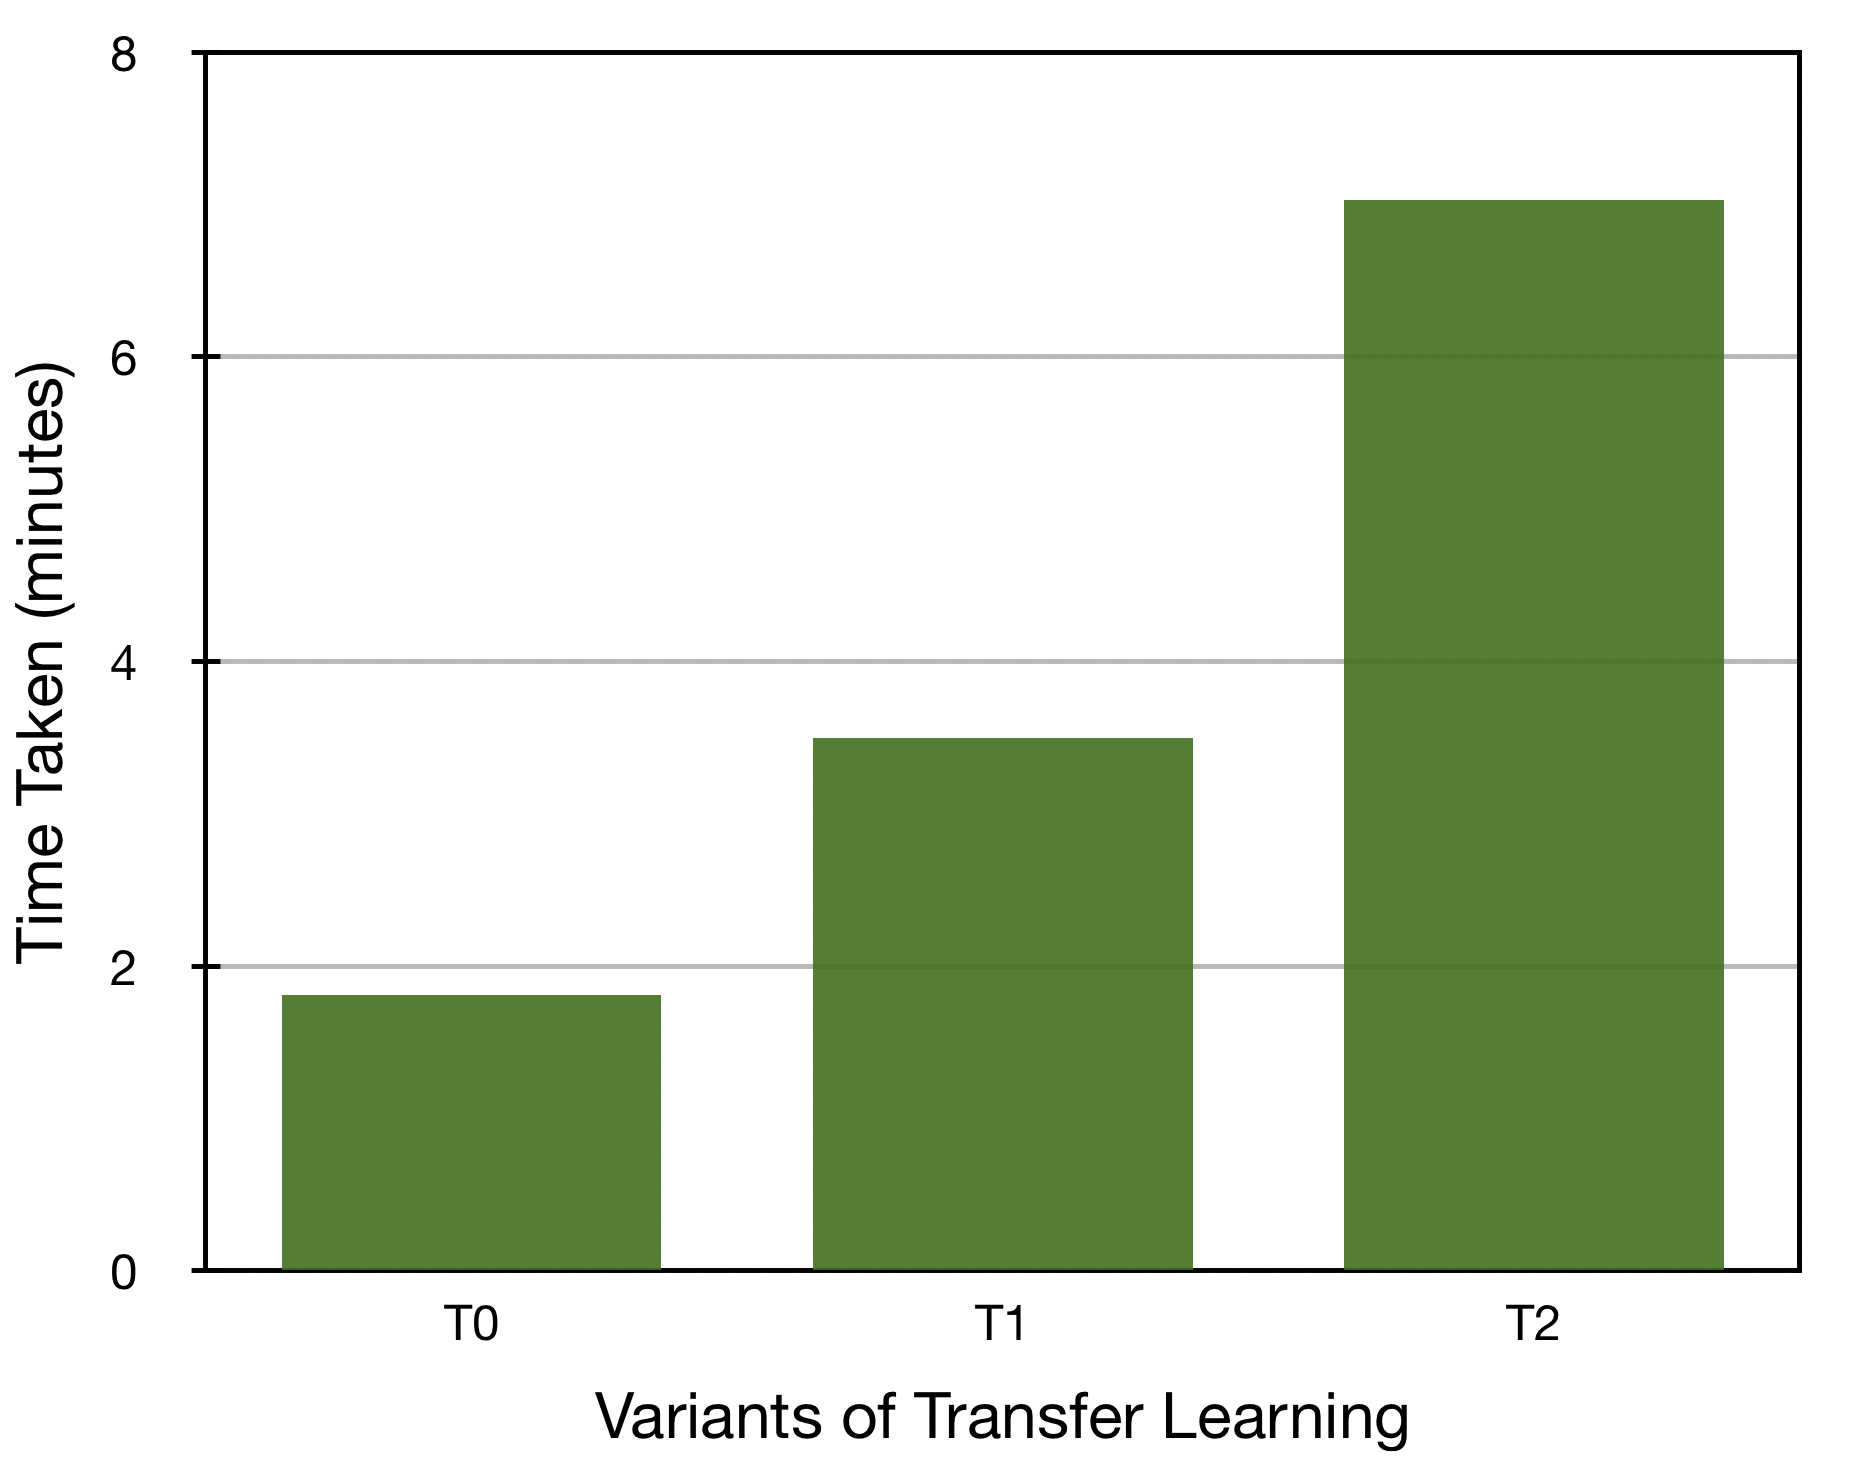
\includegraphics[width=\linewidth]{figs/time_ter.png}
   \caption{Time taken comparison}
   \label{fig:time_ter}
  \end{subfigure}
    \hfill
    \caption{Comparison of the three implementations of the transfer learning.}
    \label{fig:siatrainloss1}
\end{figure}

The next three rows show the results of the variants of the siamese network. S0 and S1 are the variants for the same model but with a different loss function. In theory and as discussed in the original paper, triplets of training data samples would outperform contrastive loss. The triplet loss tries to be less greedy than contrastive loss since the distance is a relative concept. However, it is not the case in our experiment. The one with contrastive loss results in 1.5\% better accuracy. A possible reason could be that the dataset we used is simple for classification. There are significant differences between every two categories. The one with contrastive loss, therefore, could result in a good enough performance. On the other hand, the one with triplet loss trends to be over-fitting. Finally, the implementation that we used the features from Xception and added two dense layers with the siamese network of triplets did improve the features for classification. As we see in the last row, the accuracy improved more than 4\% and 3\% when compared to S1 and S0 respectively. These results are visualized in the figure \ref{fig:acc_sia} as well. It's obvious that S2 performs best among all these three variants. Meanwhile, as shown in the figure \ref{fig:time_ter}, the variants of triplet loss took much less than the variant of contrastive loss. The training time of S2 is almost two times less than S0. The possible reason is that the model with contrastive loss requires more training data than triplet loss. The former one needs both the positive pairs and negative pairs. The anchor samples, therefore, need to be repeated two times. In summary, S2 is the one with the best performance and efficiency among these three variants.

\begin{figure}[h]
  \centering
  \begin{subfigure}[b]{0.48\linewidth}
  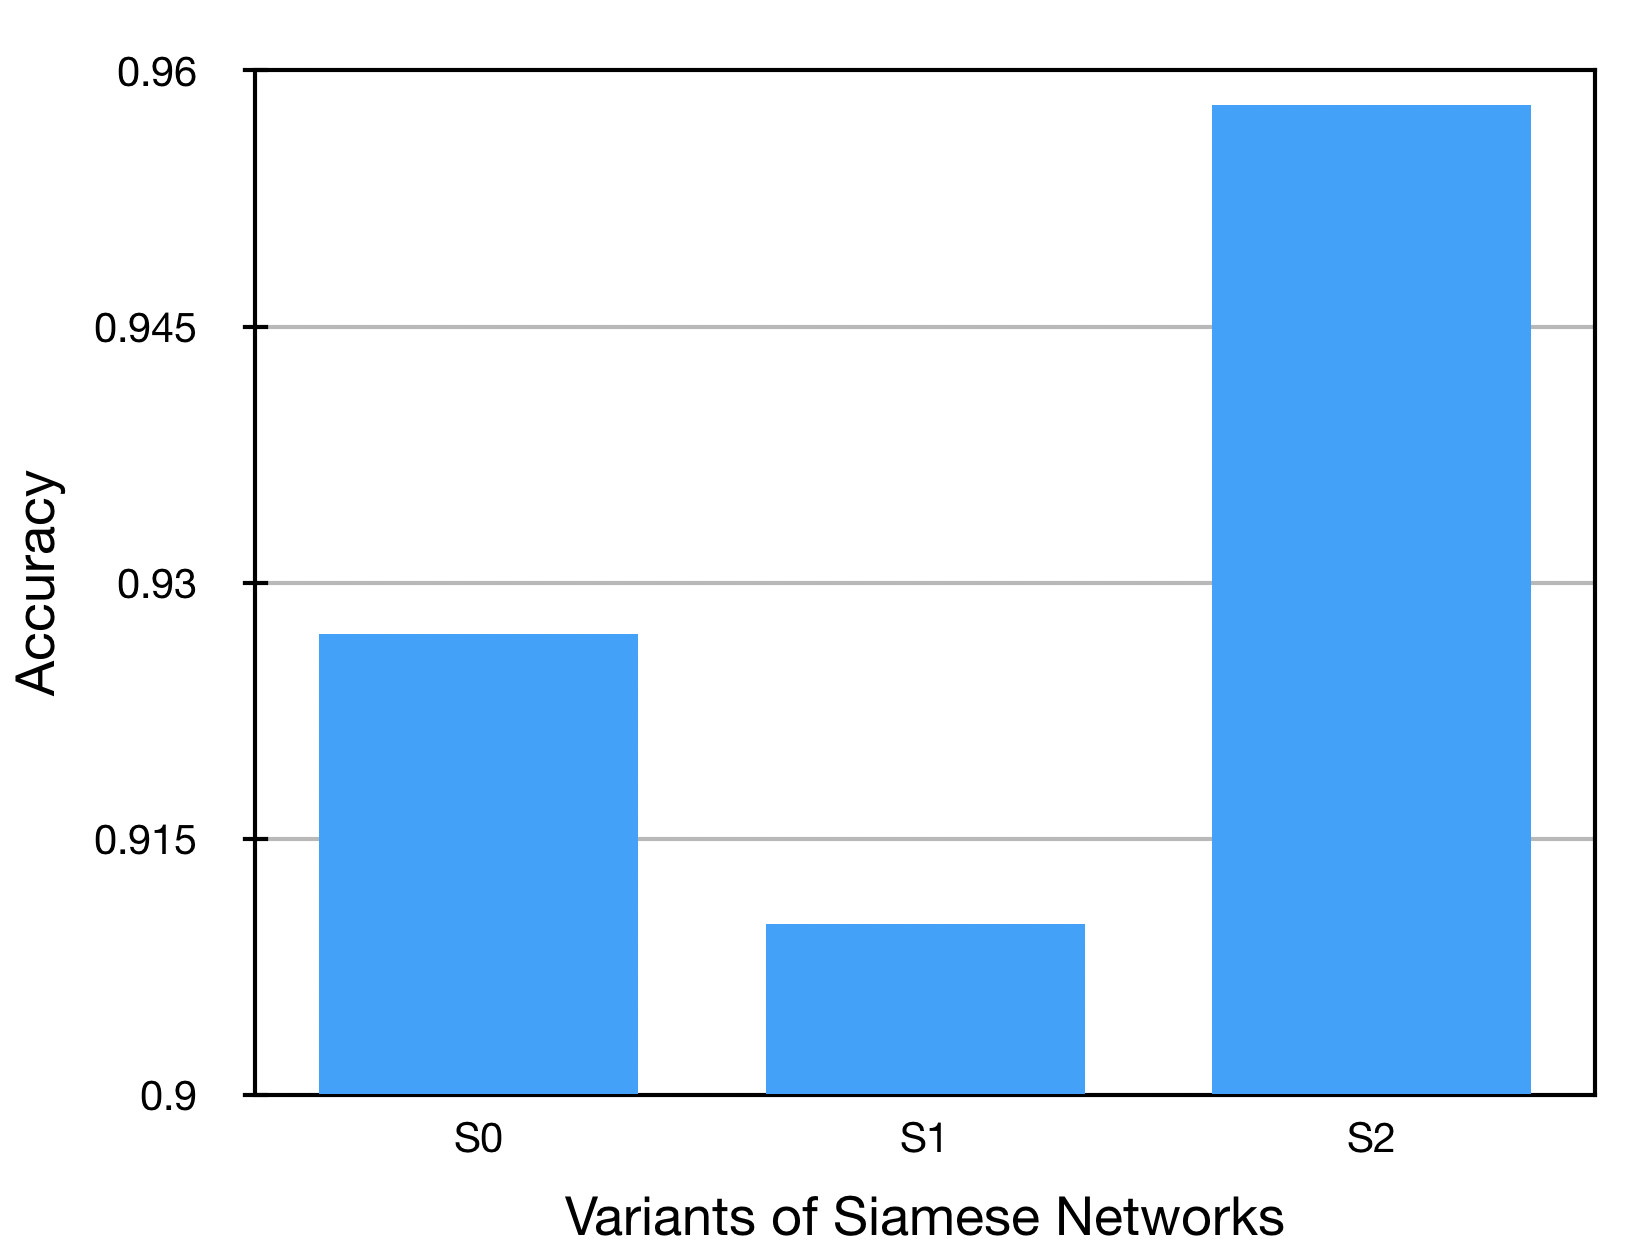
\includegraphics[width=\linewidth]{figs/acc_sia.png}
  \caption{Accuracy comparison}
  \label{fig:acc_sia}
  \end{subfigure}
  \hfill
   \begin{subfigure}[b]{0.48\linewidth}
   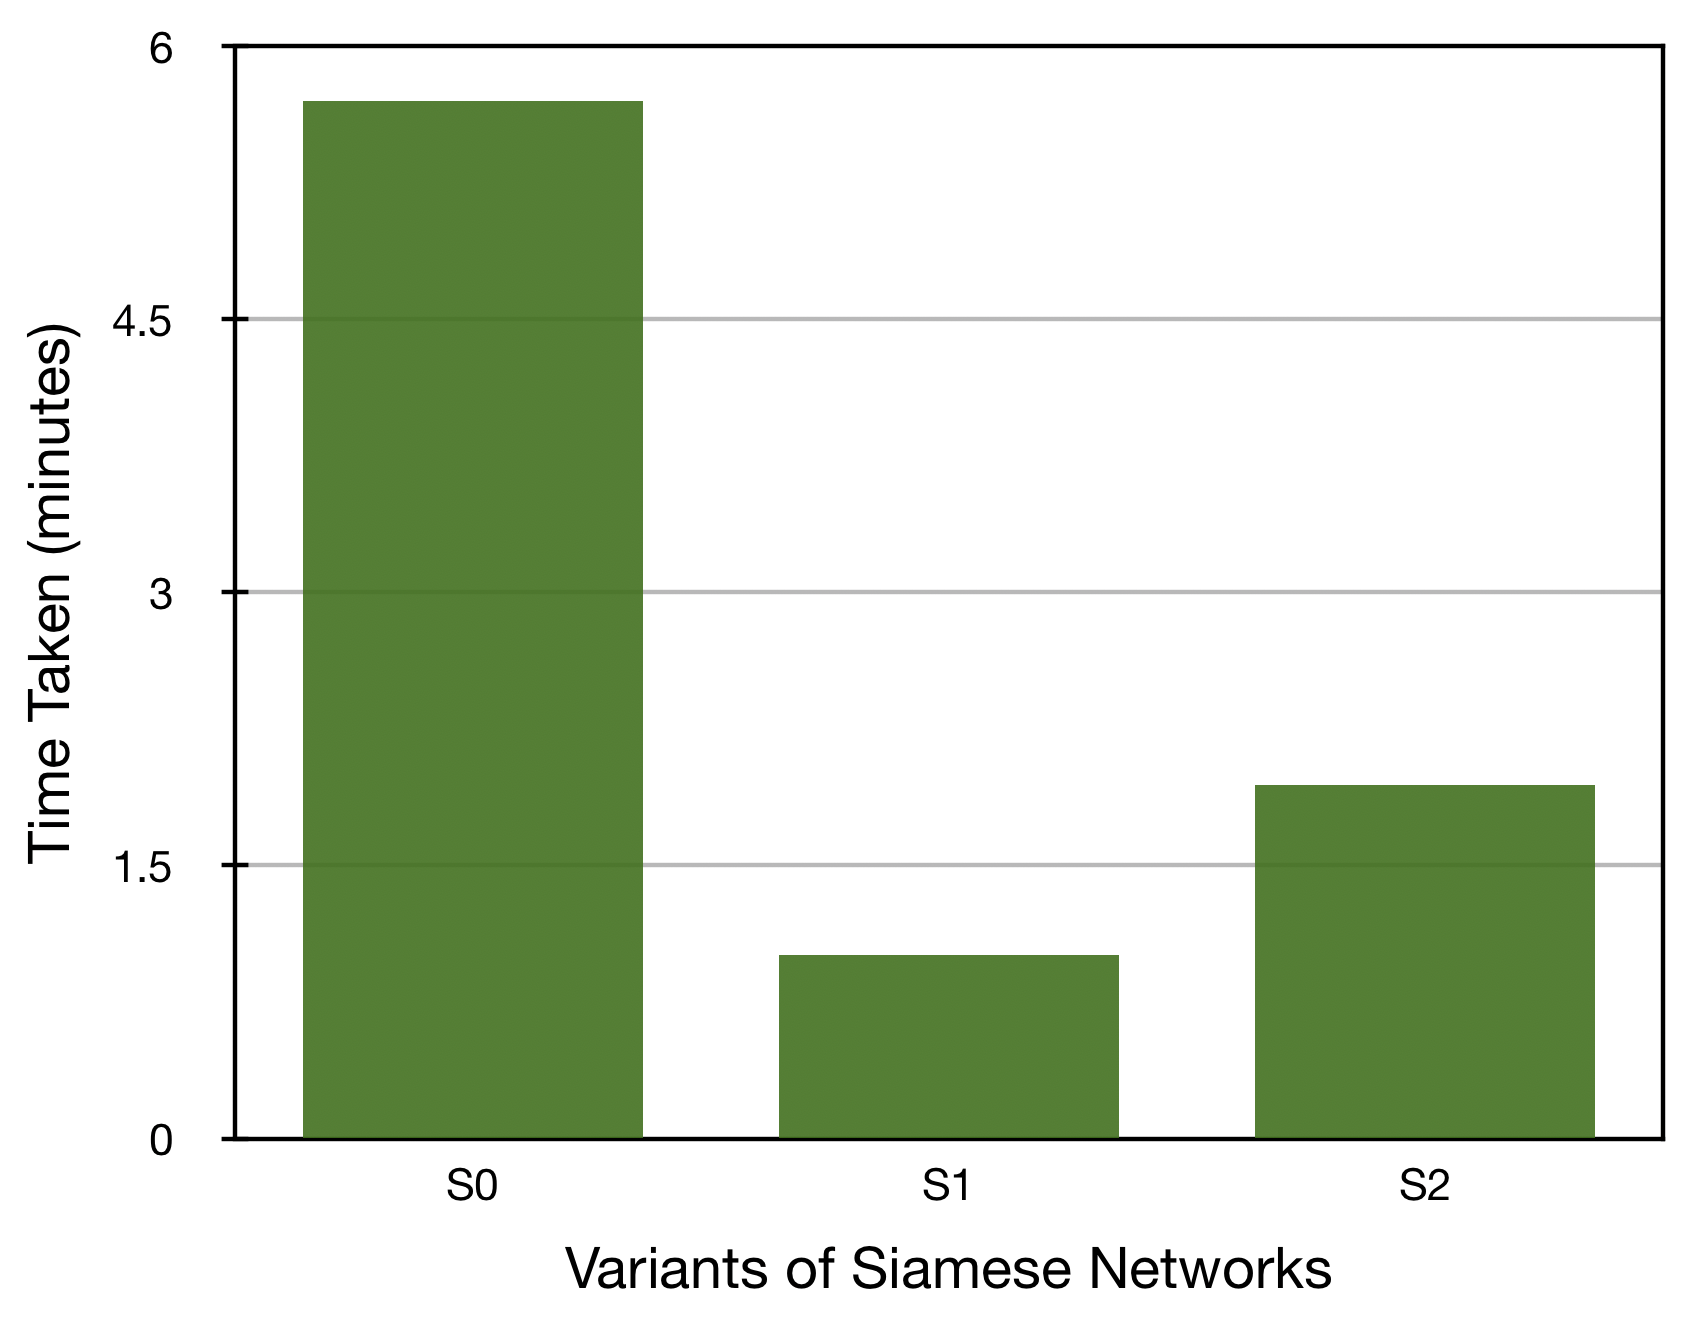
\includegraphics[width=\linewidth]{figs/time_sia.png}
   \caption{Time taken comparison}
   \label{fig:time_sia}
  \end{subfigure}
    \hfill
    \caption{Comparison of the three implementations of the siamese network.}
    \label{fig:siatrainloss2}
\end{figure}


We further compared the two best models of transfer learning and the siamese networks. We obverse that S2, the variant of the siamese network, slightly outperforms training Xception from scratch by .7\%. We can see it clearer in figure \ref{fig:acc}. Although it's not a big performance improvement, S2 spent much less time than T2, as shown in figure \ref{fig:time}. S2 reduced more than two times when compared to T2 in terms of training time-consuming. It could be very helpful in the real application, especially the situation with limited computable resources. This comparison can also be visualized in figure \ref{fig:2Dprojection}. They are two visualizations of the embedded test data projected to 2D space with UMAP using Projector from TensorFlow.  It is clear that the features of S2 are much improved and can easily be classified compared with the exception model trained from scratch. 

\begin{figure}[h]
  \centering
  \begin{subfigure}[b]{0.48\linewidth}
  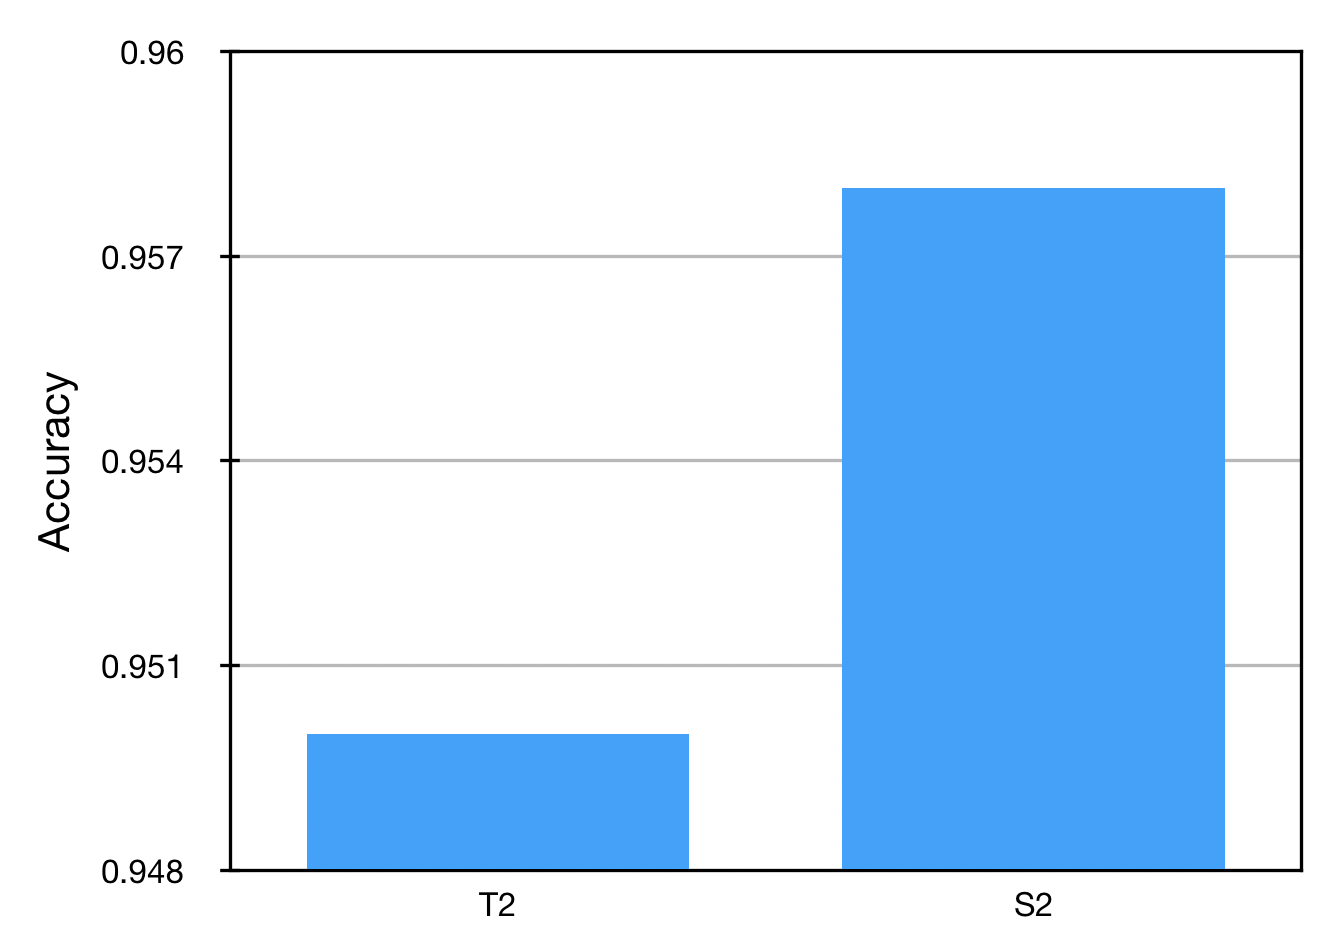
\includegraphics[width=\linewidth]{figs/acc.png}
  \caption{Accuracy comparison}
  \label{fig:acc}
  \end{subfigure}
  \hfill
   \begin{subfigure}[b]{0.48\linewidth}
   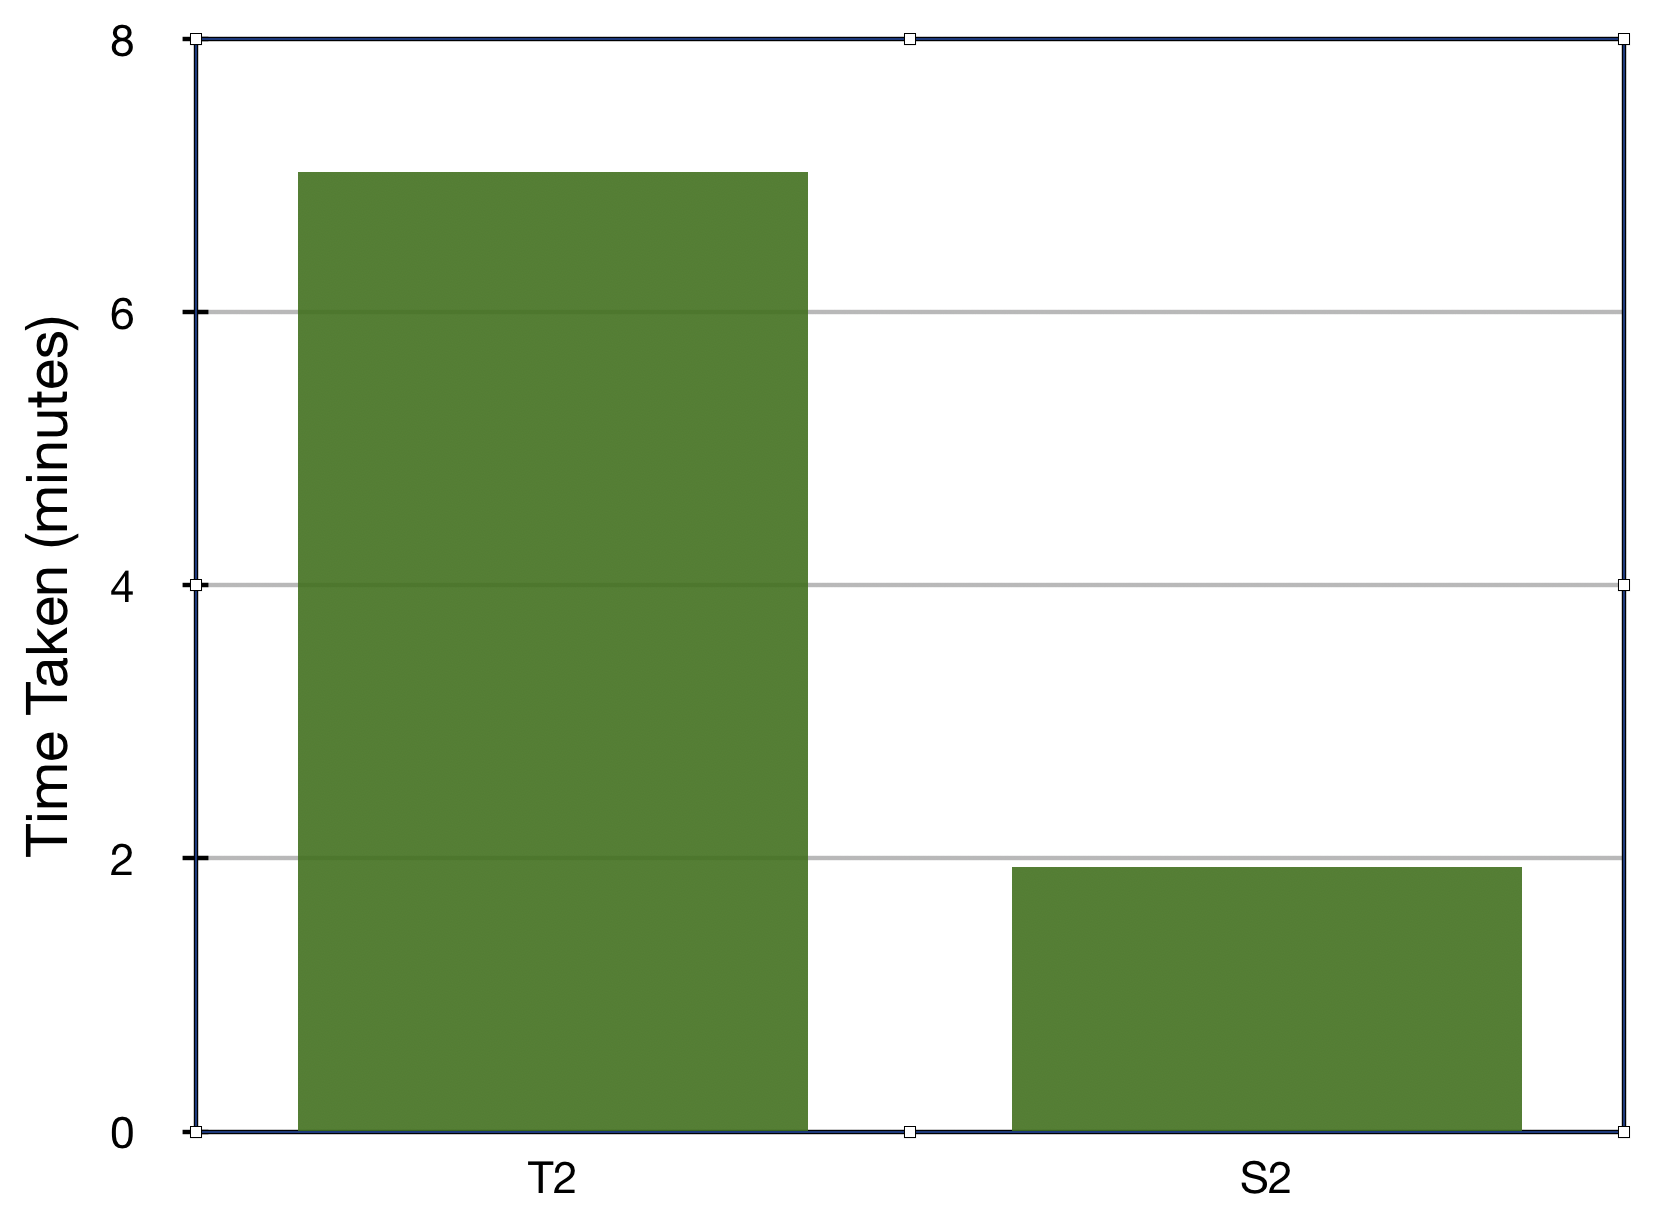
\includegraphics[width=\linewidth]{figs/time.png}
   \caption{Time taken comparison}
   \label{fig:time}
  \end{subfigure}
    \hfill
    \caption{Comparison of the two best implementations.}
    \label{fig:siatrainloss3}
\end{figure}

\begin{figure}[h]
  \centering
  \begin{subfigure}[b]{0.48\linewidth}
   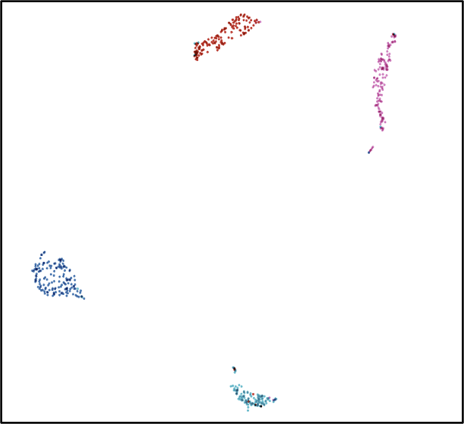
\includegraphics[width=0.9\linewidth]{figs/umab_visualS2.png}
   \caption{Xception + Siamese (S2)}
   \label{fig:tri_loss}
  \end{subfigure}
  \hfill
   \begin{subfigure}[b]{0.48\linewidth}
  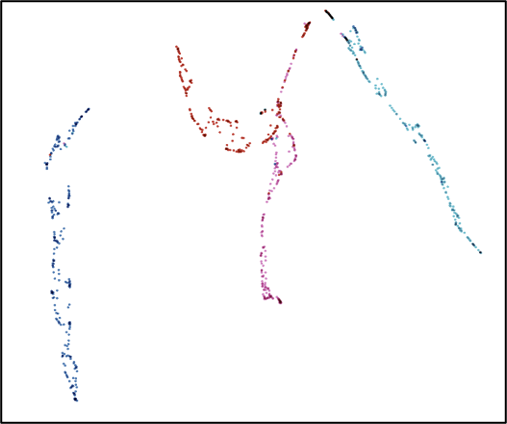
\includegraphics[width=\linewidth]{figs/umab_visualT2.png}
  \caption{Siamese all(T2)}
  \label{fig:con_loss}
  \end{subfigure}
    \hfill
    \caption{visualization of embedded test data projected to 2D space with UMAP.}
    \label{fig:2Dprojection}
\end{figure}

Besides, note that the number of training epochs of all the six variants is different. (you may give an explanation why they are different here. )


Moreover, we also trained the variants on a larger dataset that we mentioned in section 2. In this dataset, each category has 2500 images. However, we had to do some data augmentation (mirror only) for the slippers class since it only has 1283 images. Table \ref{table:resultB} shows the results. We observe that the performances of all the variants decreased when compared to the results of the previous dataset. All the performances are reduced by 1\% to 2\%. This decreased the accuracy in all experiments. We believe that it is because all the images are portrayed in the same orientation. So, using mirrored orientated images for a single class confused the models.  Figure \ref{fig:sia_con_data} further demonstrates the comparison in each category. We can see that it affected all the categories, not just the slippers.  A possible reason is that the negative samples are randomly chosen from the classes which are different from the anchor samples. Hence, the flipped images can be the negative ones for all the classes except the slippers. And the distance between the anchor sample and the negative sample would be easily larger than the margin if the negative one is the flipped image. The model then will ignore these samples. Therefore, it would give us a bad performance. In addition, from the figure \ref{fig:sia_con_data}, we can observe that the performance of the Boots category is always the best one. That's because the images of Boots are distinct from others, whereas, the images of other categories are sometimes similar to each other. 

\begin{table}[ht]
    \caption{Summary of the results on 2500 images per category} 
    \centering 
    \begin{tabular}{c c c c} 
    \hline\hline   
    model & Accuracy \% & Epochs & Time (mins)  \\% inserts table
    \hline % inserts single horizontal line
    Xception (T0) & 89.9 & 20 & 4 \\% inserting body of the table
    Xception+dense (T1) & 89.3 & 20 & 4 \\% inserting body of the table
    Xception All (T2) & 94.0 & 10 & 6 \\% inserting body of the table
    Our Siamese+Con. Loss (S0) & 90.2 & 32 & 14 \\% inserting body of the table
    Our Siamese+Triplet. Loss (S1) & - & - & - \\% inserting body of the table
    Xception+Siamese (S2) & - & - & - \\% inserting body of the table
    \hline 
    \end{tabular}
\label{table:resultB} % is used to refer this table in the text
\end{table}

 \begin{figure}[h]
  \centering
  \begin{subfigure}[b]{\linewidth}
  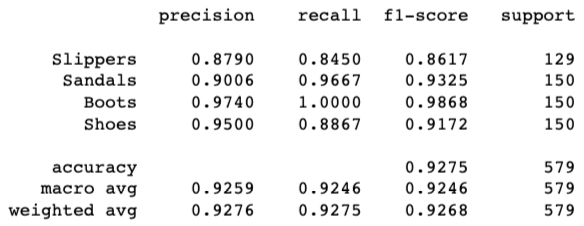
\includegraphics[width=\linewidth]{figs/sia_con_data1.png}
  \caption{Results with the dataset 1.}
  \label{fig:sia_con_data1}
  \end{subfigure}
  \hfill
   \begin{subfigure}[b]{\linewidth}
   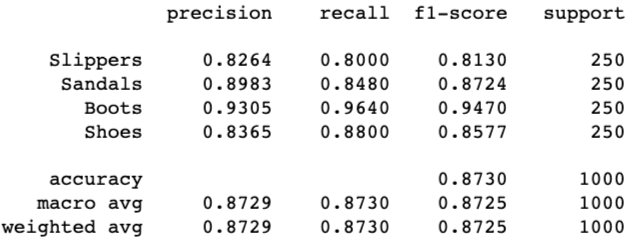
\includegraphics[width=\linewidth]{figs/sia_con_data2.png}
   \caption{Results with the dataset 2.}
   \label{fig:sia_con_data2}
  \end{subfigure}
    \hfill
    \caption{Comparison of the results of the siamese network implementation with contrastive loss with two datasets.}
    \label{fig:sia_con_data}
\end{figure}

In addition, we can also try to compute the similarity between image pairs, as shown in figure \ref{fig:similarity}. Note that the smaller distance between the two images means they are more similar to each other. For example, in the figure, the distance between the first pair in the first row is 0.10, and it turns out that they belong to the same class Slippers. As for the second pair in the same row, the class of the left image is Slippers and the class of right image is Shoes. The distance between them is 0.84, which is much larger than the first pair, as we expected. 

\begin{figure}[h]
  \centering
  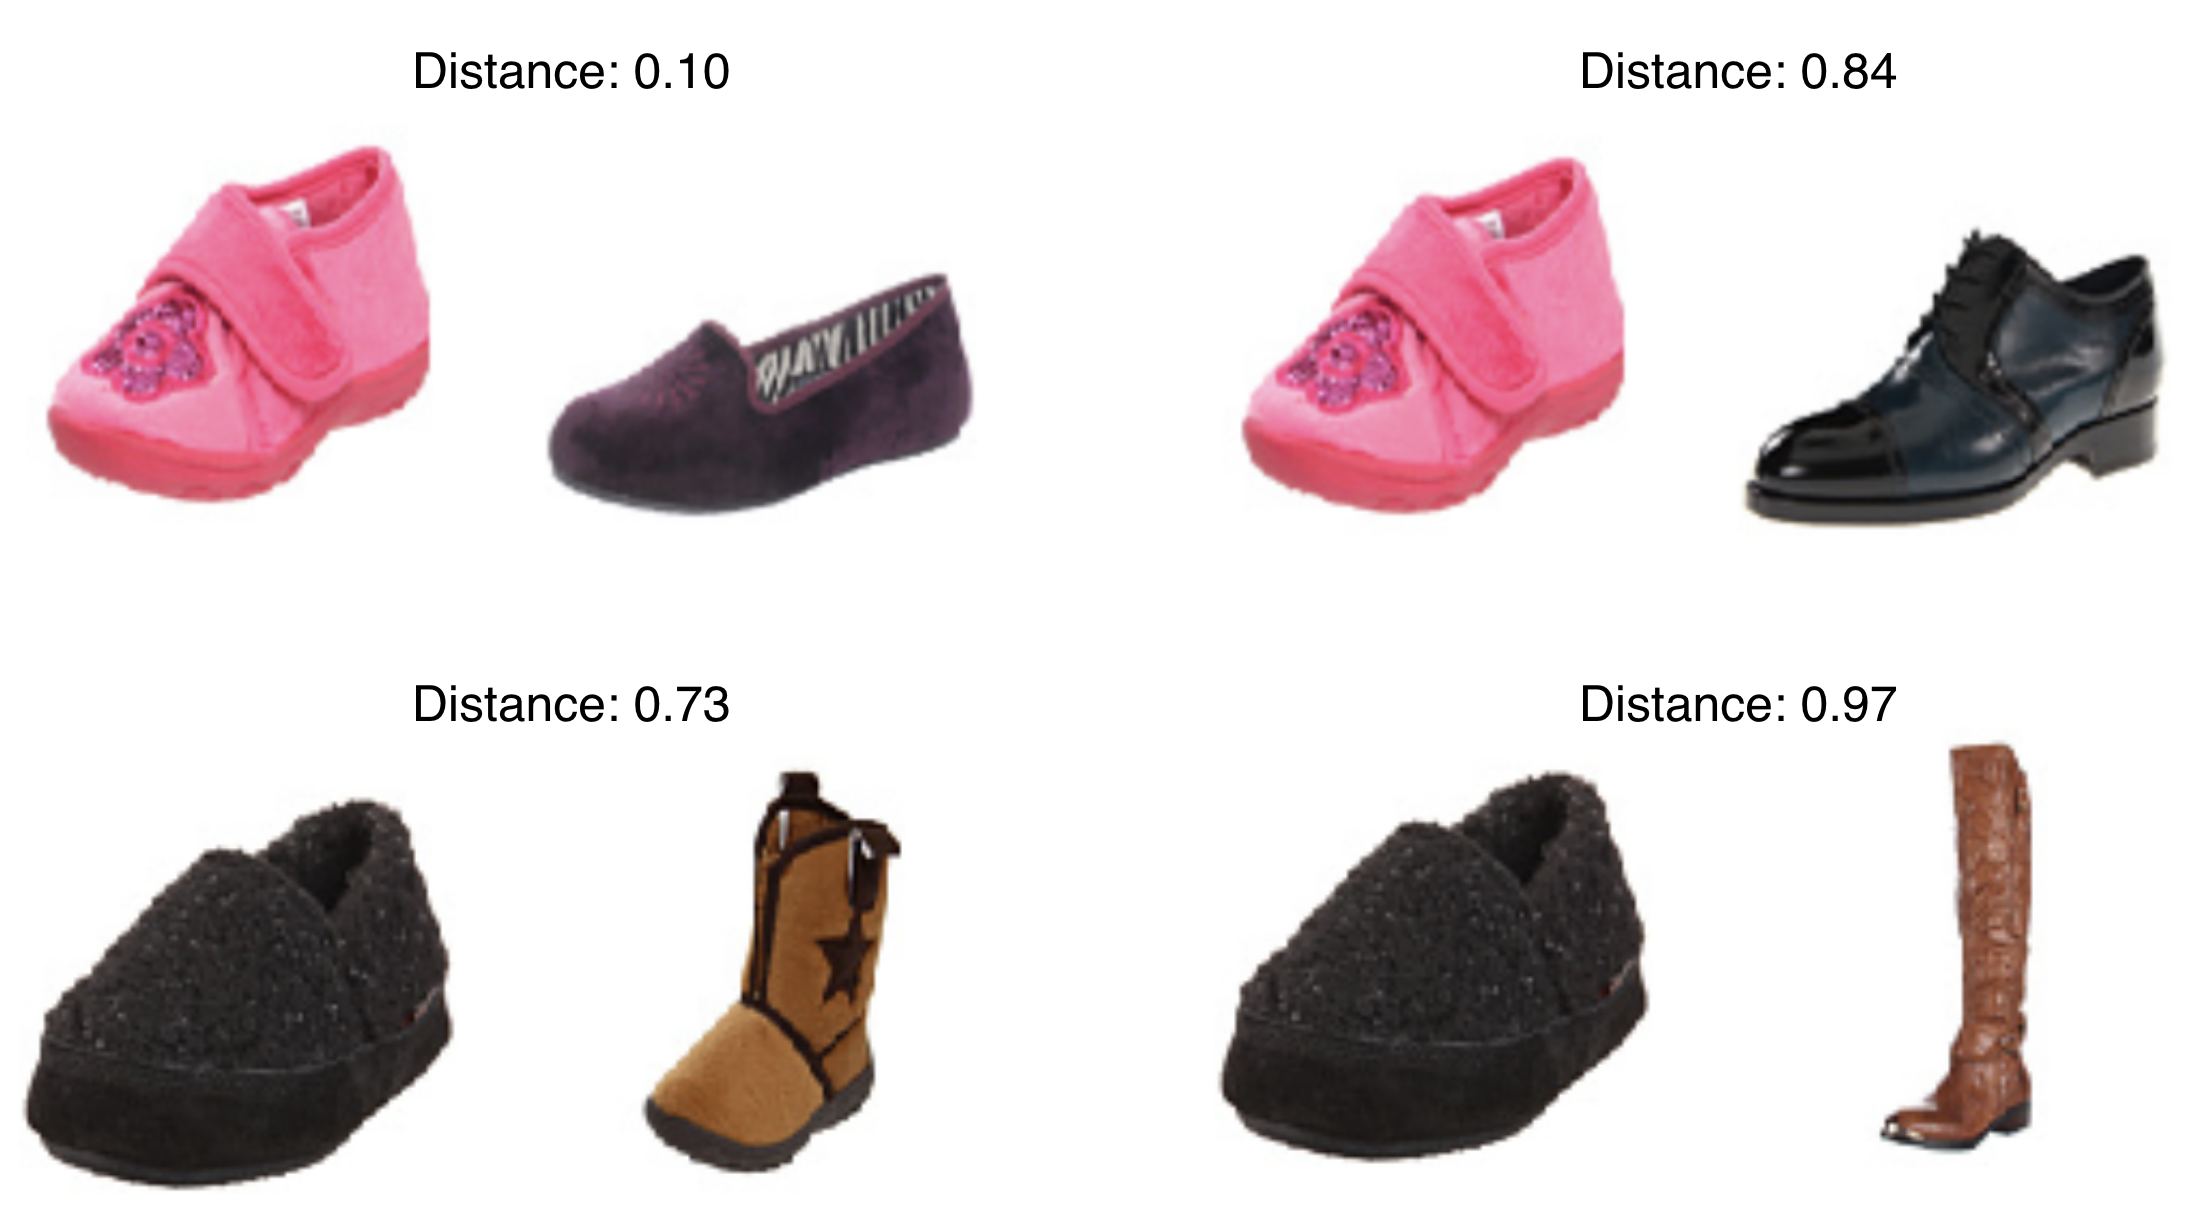
\includegraphics[width=\linewidth]{figs/similarity.png}
  \caption{Examples of calculating the similarity of image pairs.}
  \label{fig:similarity}
\end{figure}


